The previous chapters introduced fundamental concepts that allowed the development of DroidGuardian. This chapter presents their practical application on the implementation process. At first, it is introduced the environment in which DroidGuardian was built concerning operating systems and tools. Follows a detailed description of each component preceded by the general architecture. The last section highlights some relevant implementation decisions.

\section{Setting up the environment}

Building DroidGuardian comprised several stages that are directly related to the layer that was being handled. For instance, the kernel module layer requested a completely different implementation environment when compared to the Java layer.

In order to fully understand the \gls{lsm} framework it was necessary to manipulate a real Linux kernel, as well as compile it and install it. Since the development computer used was a \textit{MacBook Pro}, which runs the \textit{OS X} operating system, a new disk partition was created to install the \textit{Xubuntu} operating system. It is a different flavor of the \textit{Ubuntu Linux} operating system that provides a light user interface. Since the only needed program was the console, because all required steps could be executed through the command line and using \textit{Vim}, a lighter user interface was good enough. The new disk partition was created using the \textit{rEFIt}\footnote{http://refit.sourceforge.net} tool.

Running Linux on a new partition provided speed and efficiency when setting up the Android environment in order to build and launch a new image on the emulator. However, handling loadable kernel modules on a separate partition proved to be a mistake, due to the system's blocking when kernel failures were reached by programming errors. To overcome this inconvenience, programming tests with loadable kernel modules started to be done in a virtual machine. This way, if the code contained flaws that could led to a kernel panic, the virtual machine could easily be restarted causing no harm to the host operating system. \textit{VMWare} was used to virtualize a \textit{Xubuntu} operating system, being \textit{OS X} the host operating system.

Regarding the Android applications development environment, \textit{Eclipse} was chosen as the \gls{ide}, because is widely used, well documented and almost all issues an user may face are solved in internet forums, books and other sources.

Application testing was conducted on both the Android emulator and a real device. The device was a \textit{Commtiva z71} running Android 2.3.3, \gls{api} level 10.

\section{DroidGuardian Architecture}

DroidGuardian consists of three layers presented in \autoref{fig:dg_arch}. At the bottom lays the \textit{Kernel Module} that uses the \gls{lsm} framework to place hook functions in the Linux kernel. The remaining layers comprise the \gls{apk}: the \textit{Native Layer} and the \textit{Java Layer}. DroidGuardian uses a native library to communicate with the kernel module and to process some data before it arrives to the Java layer. The following sections describe each layer in detail.

\begin{figure}[h]
 \centering
 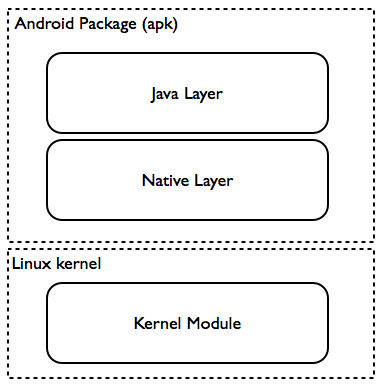
\includegraphics[scale=0.5]{figures/dg_arch.png}
 \caption{DroidGuardian architecture}
 \label{fig:dg_arch}
\end{figure}

\section{DroidGuardian Protocol}

The three layers use a protocol to communicate with each other. There are two points of communication that is important to highlight: kernel module - native layer and native layer - Java layer. Both use stream sockets to exchange data. In the first case, it is used the following structure:

\begin{lstlisting}[style=CInputStyle, caption=\texttt{security\_socket\_connect} hook (Linux kernel v3.11)]
#define DG_INET 1
#define DG_INET6 2
#define ALLOW 1
#define DENY 2
#define FOREVER 1
#define ONCE 2

struct dg_query {
  int family;
  struct sockaddr_in addrin;
  struct sockaddr_in addrin6;
  int pid;
  char process[16];
  int permission;
  int lifetime;
} 
\end{lstlisting}

The \texttt{dg\_query} structure's elements are described as follows:
\begin{itemize}
\item \texttt{family} defines the \gls{ip} version, being \texttt{DG\_INET} related to the \gls{ip}v4 and \texttt{DG\_INET6} related to the \gls{ip}v6;
\item \texttt{addrin} is used to store the address data in case of \texttt{family} is \texttt{DG\_INET};
\item \texttt{addrin6} is used to store the address data in case of \texttt{family} is \texttt{DG\_INET6};
\item \texttt{pid} gives the process ID;
\item \texttt{process} gives the process name. It is declared an array with size 16, because it gets the name from an array that has also size 16.
\item \texttt{permission} indicates if the connection is established or not, being \texttt{ALLOW} in the first case and \texttt{DENY} in the second.
\item \texttt{lifetime} assigns a time tag of the rule.
\end{itemize}

The kernel module does not inspect the \texttt{lifetime} element, because it is not responsible for creating rules. It is up to the native layer to deal with the rule's logic.

\section{Kernel Module}

DroidGuardian takes advantage of the \gls{lsm} framework in order to deny a socket connection. When a process running in the system executes the \texttt{connect()} primitive, the kernel will call \texttt{sock->ops->connect()}. Recalling the \gls{lsm} technical explanation provided in \autoref{chap:lsm} within this function is placed the security hook \texttt{security\_socket\_connect()}:

\begin{lstlisting}[caption=Code snippet of the \texttt{security\_socket\_connect} hook function(Linux kernel v3.11)]
err =
	 security_socket_connect(sock, (struct sockaddr *)&address, addrlen);
if (err)
	goto out_put;
\end{lstlisting}

If the output of the hook function is different from 0, the socket will not be connected. Therefore, the kernel module sends the \texttt{address} structure, as well as the ID and name of the process who called the \texttt{connect} primitive to the Android application, and waits for a value to return. If the connection request was accepted by DroidGuardian, the hook function returns 0, otherwise returns \texttt{EPERM}, which is the macro to \textit{Operation not permitted} and has value 1.

The kernel module implements the callback as \texttt{droidguardian\_socket\_connect()}, which is responsible for sending the socket data to the Android application. It fulfills this task by calling auxiliary functions that set up a stream socket client and preparing a query structure to be filled in. \autoref{fig:kernel_module_flow} presents the kernel module flow diagram.

\begin{figure}[h]
 \centering
 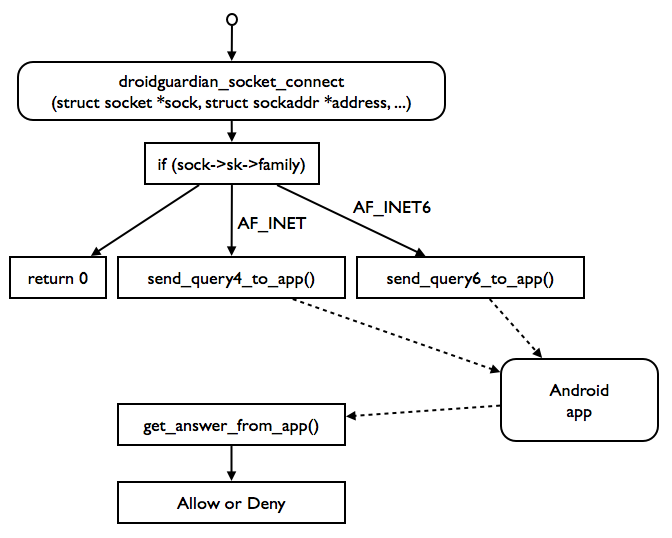
\includegraphics[scale=0.5]{figures/kernel_module_flow.png}
 \caption{Process flow in the kernel module}
 \label{fig:kernel_module_flow}
\end{figure}

The hook function receives three arguments:
\begin{itemize}
\item \texttt{struct socket *sock}
\item \texttt{struct sockaddr *address}
\item \texttt{int addrlen}
\end{itemize}

The first structure contains the data regarding the socket that is trying to connect to a server socket. The second structure contains the server address to which it intends to connect. Note that the \texttt{connect()} primitive was introduced in \autoref{sec:sockets}. Once the hook function is called, these arguments are inspected:

\begin{enumerate}
\item The socket family type is analyzed. In case it is different from \texttt{AF\_INET} or \texttt{AF\_INET}, the hook function immediately returns 0 allowing the connection. DroidGuardian is only interested in filtering internet sockets. Furthermore, DroidGuardian uses unix domain sockets. If they were intercepted as well the function would enter a dangerous loop.

\item Once passed the family type check, \gls{ip} versions are distinguished: if the socket is specified as \gls{ip}v4 (\texttt{AF\_INET}) a \texttt{sockaddr\_in} structure is filled in by casting the \texttt{sockaddr} argument; otherwise the socket concerns \gls{ip}v4 (\texttt{AF\_INET6}) and a \texttt{sockaddr\_in6} structure is filled in, in the same way. These structures will store the server address data that will be sent to the application.

\item Along with the server address, the process that launched the connection request needs to be identified. At kernel level, it is possible to use the \texttt{current} global variable that points to the \texttt{ task\_struct} structure provided by the \texttt{include/linux/sched.h} header file. This structure contains the data related to the running process. Using \texttt{current->pid} and \texttt{current->comm} it is possible to get the process ID and name, respectively. These data also is sent to the application.

\item A new client socket (unix domain) is created to communicate with the application, and the subsequent steps to establish a stream connection are executed.

\item The \texttt{sock\_sendmsg()} function is called to send the data to the application.

\item At last, the \texttt{sock\_recvmsg()} function is called to get the value that will define the hook as permissive or blocker.
\end{enumerate}

\section{Native Layer}

As explained before, Android developers are provided an interface to take advantage of the powerful native libraries. DroidGuardian uses this power to bridge the communication between the kernel module and the Java application. \autoref{fig:dg_native_flow} presents the process flow of the native layer.

\begin{figure}[h]
 \centering
 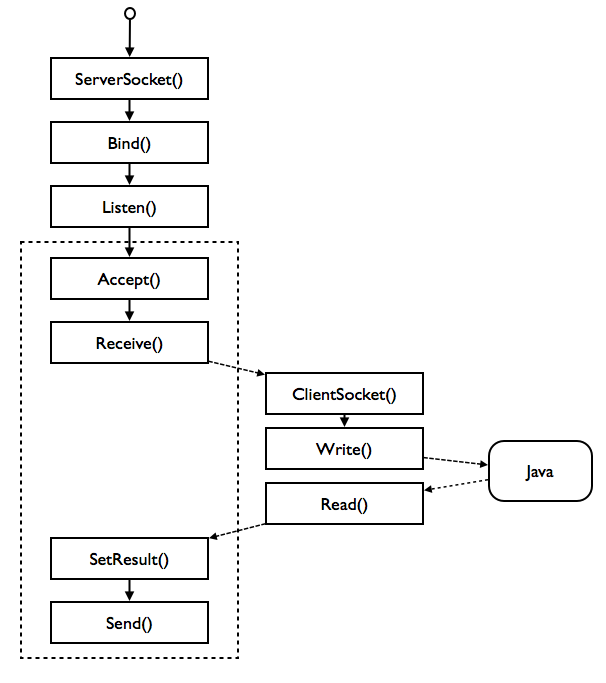
\includegraphics[scale=0.5]{figures/dg_native_flow.png}
 \caption{Process flow in the Native layer}
 \label{fig:dg_native_flow}
\end{figure}

The native code is executed as a native library by the Java application. Therefore, is the Java layer that calls the native library. Once this happens, the main native function \texttt{startDaemon()} starts its execution. It fulfils two main goals: act as a server to communicate with the kernel module and act as a client to communicate with the Java layer. In the former, the native code follows the common protocol to establish a stream socket connection, as creating the socket, binding to a local address and listening to client requests. Once the server socket is listening, it enters an infinite \texttt{while(1)} loop to be always ready to accept requests. Inside the loop, it eventually accepts a client request that comes from the kernel module and exchanges data with this. The native server socket is able to get the query through the \texttt{read()} primitive. This query is analyzed and according to the family field (\texttt{DG\_INET} or \texttt{DG\_INET6}), the function \texttt{query4\_to\_java()} or the function \texttt{query6\_to\_java()} is executed, respectively. These functions extract the \gls{ip} address and port from the \texttt{struct sockaddr\_in} or \texttt{struct sockaddr\_in6} passed in the query, along with the pid and process name, and send this data to the Java layer through a client socket connection. 

The second goal is reached at this point. The native layer contains the data sent by the kernel module and needs to drive it to the Java layer. Once again, sockets are used to achieve this goal. Since Java local sockets in Android only use abstract namespaces, the client socket created in the native side use an abstract namespace as well. In order to get the input stream that Java provides through the \texttt{InputStream} \gls{api}, all data needs to be wrapped up as an unique string. This string is sent to the Java layer through the \texttt{write()} primitive and the response is received through the \texttt{read()} primitive.

\section{Java Layer}

The topmost layer of DroidGuardian has the only purpose of displaying the data to the user. This is achieved through an Android application, that is provided with both the necessary components and a powerful \gls{api}. Android components, presented in a previous chapter, were carefully studied in order to ensure that DroidGuardian was being built with the proper pieces. However, when compared to the usual Android applications lifecycle, DroidGuardian may be seen as a different kind of application that was not though to follow the good tips when it concerns the behavior of applications in mobile environments. But, more on that later.

\begin{figure}[h]
 \centering
 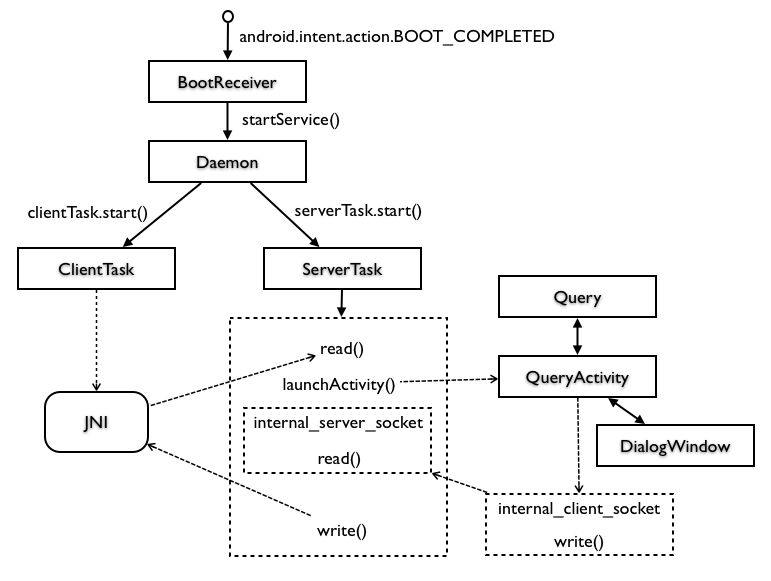
\includegraphics[scale=0.5]{figures/dg_java_flow.png}
 \caption{Process flow in the Java layer}
 \label{fig:dg_java_flow}
\end{figure}

The process flow of the Java layer is illustrated in \autoref{fig:dg_java_flow}. It presents the following classes:

\begin{itemize}
\item \texttt{BootReceiver}: operates as a \textit{BroadcastReceiver} that starts DroidGuardian after the device booting process.
\item \texttt{Daemon}: acts as a \textit{Service} to run in background while the device is on.
\item \texttt{QueryActivity}: is the \textit{Activity} responsible for displaying the data of queries to the user.
\item \texttt{Query}: does not extend an Android component, being used to translate a native query into a Java query.
\item \texttt{DialogWindow}: is bounded to the \texttt{QueryActivity}, building a fragment to display the dialog window.
\end{itemize}

DroidGuardian was design to run as a daemon, silently and unnoticed, until internet connection requests arose to trigger the dialog window.  Also, applications may launch internet requests at any time since the device starts running. Therefore, DroidGuardian needs to start listening as soon as possible. Android fires an intent immediately after the booting process, allowing applications to receive it:

\indent \texttt{android.intent.action.BOOT\_COMPLETED}

This intent is received trough \textit{Receivers} or \textit{BroadcastReceivers} that overwrite a callback named \texttt{onReceive()}. This method is responsible for grabbing intents and triggering whatever action the developer wants. In this case, the \texttt{BootReceiver}'s \texttt{onReceive()} method starts the daemon allowing DroidGuardian to connect to the kernel module and start listening internet requests.

The following steps describe the process flow of the Java layer:

\begin{enumerate}
\item Android sends \texttt{BOOT\_COMPLETED} intent action and \texttt{BootReceiver} grabs it.
\item \texttt{BootReceiver} starts the service \texttt{Daemon} after grabbing the intent.
\item The \texttt{Daemon} service launches two threads: \texttt{ServerTask} and \texttt{ClientTask}. The former operates as a server in the stream socket protocol and will run until an external perturbation, as low memory, destroys the service. If nothing happen, this socket server will run while the device is on. The last acts as the client socket in this connection. However, the client code is not implemented in this class but in the native library. This thread calls the native method \texttt{startDaemon()} that kicks off the native engine.
\item Once executing, the server socket starts a \texttt{while(1)} loop in which queries' data will be exchanged between the server and the client.
\item When the client gets a query sends it to the server, that receives it through the \etxttt{read()} method of the \texttt{InputStream} interface.
\item Immediately after reading the query, the server invokes an instance of the \texttt{QueryActivity} class through intents, transmitting the query's data.
\item Along with this call to \texttt{QueryActivity}, the server also initializes a new server socket, called internal server, that will handle the communication between the \texttt{Daemon} and the \texttt{QueryActivity}.
\item The \texttt{QueryActivity} gets the query's data in a special format. Then, creates an instance of the \texttt{Query} class, which has as instance variables the fields that will ultimately display the information to the user.
\item This process culminates with the execution of the \texttt{DialogWindow}. The \texttt{QueryActivity} instantiates a new Activity Fragment and exhibits it through the \texttt{show()} method.
\item The \texttt{DialogWindow} fills itself with a View that contains a text, a spinner and buttons. The text displays the internet connection request information so that the user may decide what option to chose in the spinner and what button to click on.
\item Once the user clicks a button, the \texttt{DialogWindow} executes a method that provides from a Java Interface and is implemented in the \texttt{QueryActivity} class. This method starts the internal client socket that will send the user's action to the internal server, listening on the \texttt{Daemon}'s server loop. After sending the message, the internal client closes itself.
\item The internal server gets the information, stores it in a variable and closes itself.
\item At last, the server reads this variable's value and sends the message back to the native client.
\item This process is repeated every time a new connection request reaches the Java layer.
\end{enumerate} 

\section{Decisions}

While developing DroidGuardian, various doubts and questions came out regarding the best way to implement certain features. This section presents those cases along with the decision taken and its explanation.

\subsubsection{Dialog vs Notification}

The dialog window don't follow the correct rules that Android states when it comes to alert the user that some event occurred. Dialogs exist for this purpose, but in a different context. A dialog alert should be used inside an activity that the user intentionally invoked. For instance, when the user triggers an action to delete data from a certain folder it is expected that a dialog window pops up asking if he intends to delete that data. This is a consequence of the user's action.

In situations where an event occurs outside the application that the user is interacting with, Android offers the \textit{Notification} interface. Notifications are messages displayed on the notification bar, placed at the top (or bottom) of Android devices, by icons. When a new icon appears on the notification bar, it means that some event took place as a result from a background action. The user is able to expand the notification bar to check all notifications that, usually, comprise some short information text. By clicking on the notification area, it may fill the screen with data related to the event that occurred, depending on how the notification was developed. Users are free to keep notifications unread for as long as they want, without lose performance.

Considering both elements, dialogs and notification, the DroidGuardian case fits better in the last, because the event that triggers an alert to the user happens in background. However, taking the internet connection request to the notification bar would lead to a longest response time when compared to the dialog. The time the user takes to provide his input is included in the total amount of time that the socket waits in the kernel in order to accept or reject the connection. It is known that kernel operations should be executed as fast as possible and that keeping the kernel stuck could bring several damages to the system. Even though it is kept waiting a considerable amount of time using dialogs, compared to notifications this time would increase. 

It was decided that disrupt the user from whatever he is doing, with an alert pop up was better than keeping the kernel waiting long periods of time.

\subsubsection{Service and Activity communication}

\subsubsection{}
(FALTA ACABAR) 